\documentclass[11pt]{article}

\usepackage{multirow}
\usepackage{subfig}
\usepackage{xcolor}
\usepackage{listings}
\usepackage{graphicx}
\usepackage{amsmath}
\usepackage{hyperref}

\title{\textbf{Major Project Documentation}}
\author{Joe Withers}
\date{}

\begin{document}

\maketitle

\tableofcontents
\newpage

\section{Introduction}

This document serves to detail the work I was responsible for during the Final Major Project assignment, in which I helped create an animated short film as part of a four person team.
As an aspiring software developer, my responsibilities for this project were mainly the technical aspects within production, such as pipeline management and character rigging.

\section{Pipeline Management}

\subsection{Requirements}

\begin{itemize}

\item Reliably store all of the project data in such a way that is accessible to all team members.

\item Provide artists with a tool that manages assets, allowing them to update, reference,

\item Provide artists with a simple method for releasing new versions of assets.

\item Provide artists with a simple method for gathering assets, so that they can be referenced into a scene.

\item Manage versioning of assets, accompanied by information regarding each versions release date, author, and  description.

\item Automatically update references to assets whenever an asset or one of it's depenencies has been updated.

\item Provide an automated method for caching the entire scene, with the aim of 'packaging' the project to make it suitable for rendering on different machines.

\end{itemize}

\subsection{Limitations}

Prior to developing the pipeline and associated tools, it was important to address the limitations imposed by the environment in which we would be working. The most important of these were:

\begin{itemize}

\item Lack of unified storage amongst users. Due to the way the university network is set up, it isn't possible to have a single network location for our shared data storage, without sacrificing one members allocated user storage.

\item Lack of storage per user. The approximate storage limit per user is 50gb, which would quickly be hit in a complex production environment. It is therefore imperative that we are concious of the data that we keep hold of.

\item Lack of storage space on the renderfarm. The approximate storage limit on the renderfarm is 30gb, meaning that all of the data required to render a scene or shot must fit well within this limit, as rendered frames are written to the same location.

\end{itemize}

\subsection{Storage}

For file storage we chose to use Resilio Sync, a peer-to-peer file synchronization service
to store all of our working files. This ensured that each team member has their own local copy of the entire working directory, which is beneficial when creating backups. We chose Resilio Sync primarily because it is a free service that is compatible with the university computer network, however it does present us with some problems.

Due to being it peer-to-peer service, we often found that directories would fail to synchronize properly if not syncronized frequently with the other peers. This would not be a problem in a cloud hosted service as the directory state of the working directory would be reliably centralized, reducing the possibility of files becoming desynchronized, however these services are typically expensive and it was difficult to predict our exact storage requirements.

We also noticed a strange problem with Resilio Sync, in which the contents of files would be reduced to 0 bytes. Fortunately the data is usually not lost as it is sent to the 'Archive', which functions as a temporary recycle bin, though restoring these files manually each time it happened proved to become quite tedious. I decided to write a simple bash script to check through the working directory to identify any files with a size of 0 bytes, and to check if a matching file was present in the Archive. However, this wasn't particularly effective as often they would be missing from both the main working directory and the Archive, meaning I would have to search through backups to find the file to restore, which at times felt a bit like baby-sitting.

\subsection{Asset Management}

\subsection{Asset Pipeline}

\section{Character Rigging}

\subsection{Requirements}

For this project I was responsible for the rigging of both characters, as well as the rigging of any props that the characters interact with. Prior to working on the character rigs, it was important to outline features that would be required to achieve an appealing animation. This ranged from features that would allow the animator (Yves Bedenikovic) to work with them more efficiently, to features that would improve the overall aesthetic of the animation such as cloth and hair simulation. The following features were found to be of highest importance:

\begin{itemize}

\item Controls should be familiar to the animator to allow them to work intuitively with the rig. This can be achieved by using previous rigs that the animator has used as reference when setting up controllers.

\item Rigs should be capable of achieving the desired facial expressions and poses as dictated by the story.

\item Rigs should include the necessary geometry and nodes to allow for cloth simulation to be applied to clothes.

\end{itemize}

\subsection{Solution}

With these features in mind, I decided to use an automated rigging system to speed up the creation of the character rigs. This allowed me to focus primarily on the features listed above, and let a tool automate the creation of the basic bipedal rig.

I first looked at Kraken\cite{kraken}, a rigging system included within Fabric Engine. This appealed to me as it was easily extensible through it's scripting language, which I thought I would find intuitive given that I had produced a basic automated rigging system for the specialism assignment in second year. Unfortunately, Fabric software went bankrupt at the beginning of the academic year so we were unable to get it working on the university computers.

I then found Advanced Skeleton 5\cite{advancedSkeleton}, an extensive rigging tool for Autodesk Maya, which I found to be extremely capable and was more than adequate for my needs.

\section{Groom}

Xgen stuff

\subsection{Pipeline}

\subsection{Results}

\section{Rendering}

\subsection{Optimisation}

\subsection{Distributed Rendering Tools}

Due to inconsistencies with the renderfarm, our only other immediate option for rendering was to use the computers in the teaching labs. To maximise our rendering output and to minimise disruption to other students, I decided to connect to other computers remotely over SSH. This allows me to connect to far more computers than I would be physically able log into, and at the same time allows other users to log into and use the same computer.

> downsides
	> slow network throughput
	> unreliable (people turn pc off)

> upsides
	> hella fast

\cite{pssh}
\cite{martin_2008}

\section{Compositing}

In addition to being responsible for rendering, I took responsibility for compositing the shots, which was convinient as I was managing the storage of the raw renders and would be the first member of the team to get a chance to do any compositing. Being more technically inclined my compositing responsibilities mainly consisted of:

\begin{itemize}

\item Reconstructing the 'beauty' pass from the individual AOV passes. The AOVs we ended up using for reconstruction were direct diffuse, direct specular, indirect diffuse, indirect specular, subsurface, and transmissive, with the beauty pass being used for reference. The albedo pass was also used to generate a high pass filter for overall sharpening.

\item Rotopainting out any visual errors if time did not permit re-rendering a shot. This primarily consisted of hiding any intersections between the shirt and the jacket, or intersections between the cornea and the eyelid when the eyes were closed.

\item Removing Fireflies or any high variance visual noise from the individual passes, either through use of Nuke's denoiser or a third party 'Firefly Killer' gizmo found online \cite{muller_2015}.

\item Setting the display colour space as ACES Filmic, and setting up a node to bake the colour space prior to writing.

\item Adding depth of field to shots where depth of field wasn't calculated in RenderMan.

\end{itemize}

As these tasks were common to all shots, I created a template Nuke script which configures everything for me. Unfortunately, when reading multichannel EXRs generated by Renderman, Nuke would swap the alpha channel with the red channel from the direct specular. However this was easily fixed using a pair of copy nodes.

\begin{figure}[htbp]\centering
	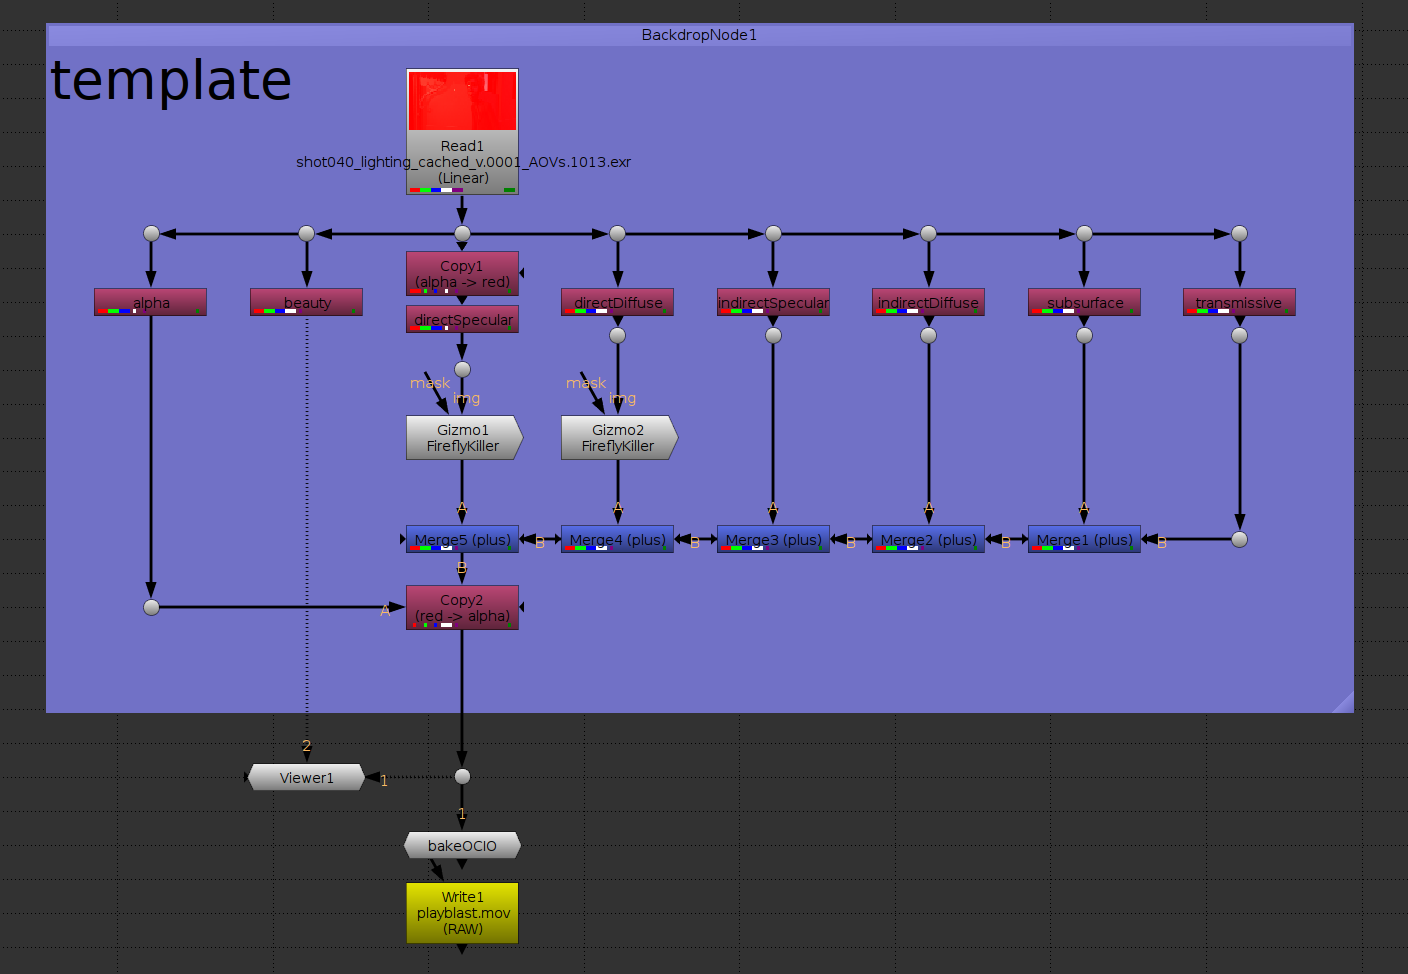
\includegraphics[width=1.0\linewidth]{images/compTemplate.png}
	\caption{\label{figure:compTemplate} The template Nuke script which was used as the basis for all shots.}
\end{figure}

For the opening shot, a more complex Nuke script was necessary as we needed to integrate FX elements, all of which were rendered seperately. We also chose to render the foreground and background seperately so that we could make adjustments to them independently.
\begin{figure}[htbp]\centering
	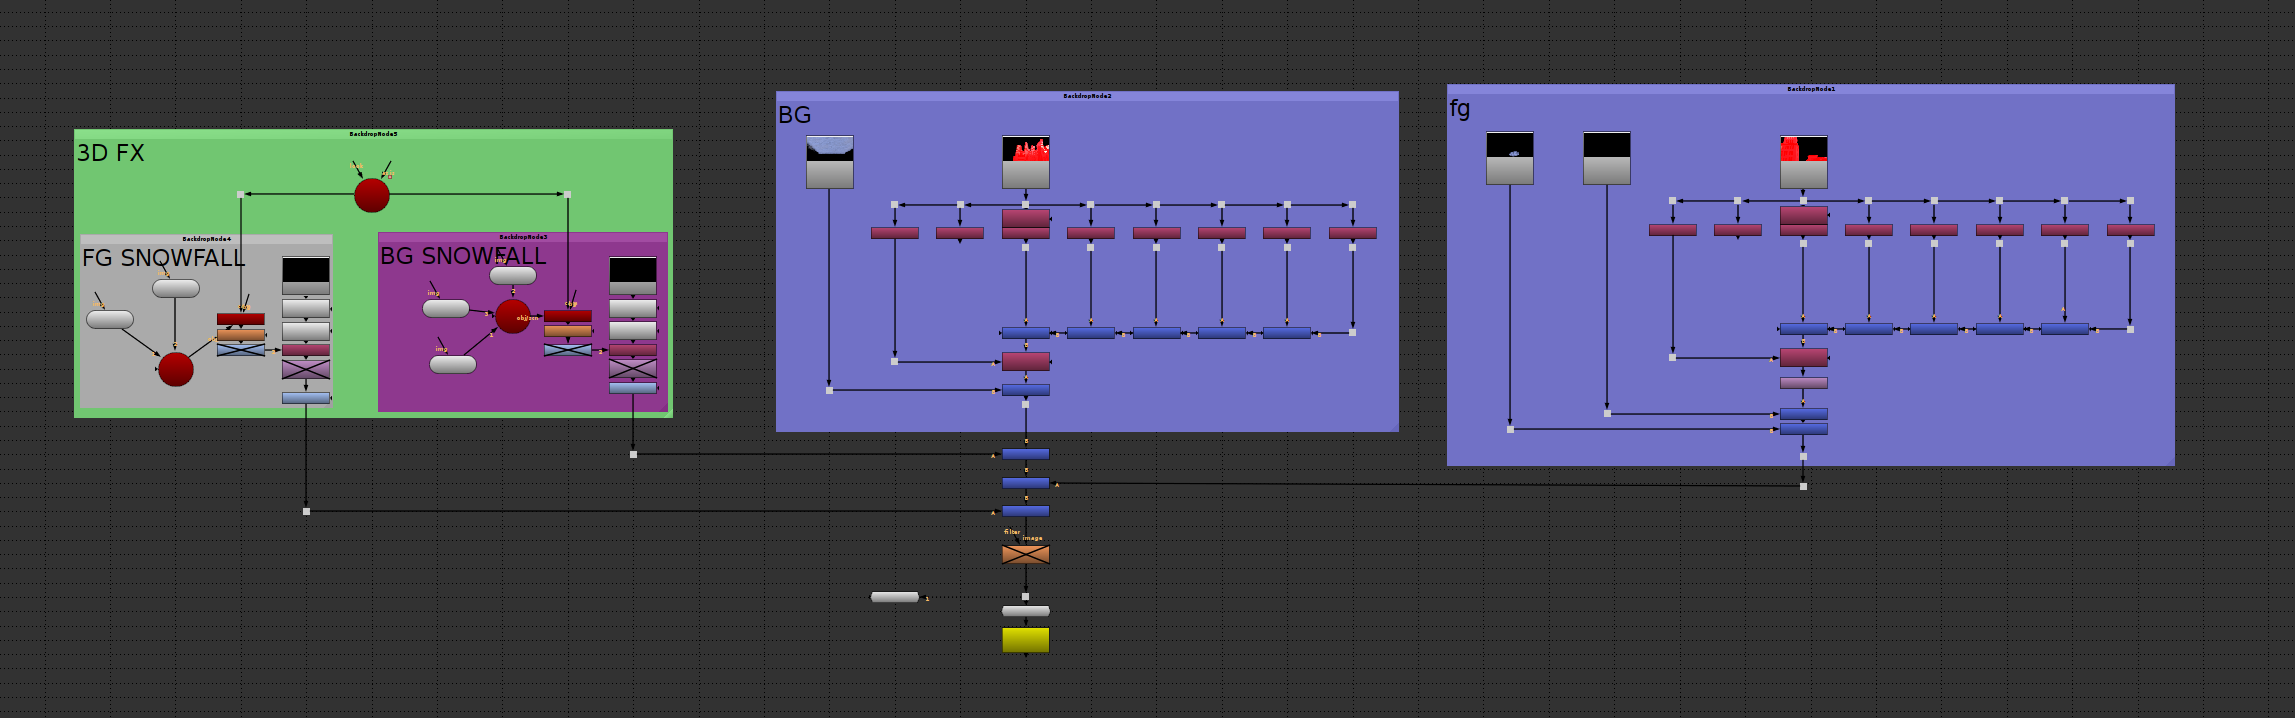
\includegraphics[width=1.0\linewidth]{images/shot010comp.png}
	\caption{\label{figure:shot010comp} The Nuke script which was used for the opening shot.}
\end{figure}

\bibliographystyle{plain}
\bibliography{references}

\end{document}
